%%%%%%%%%%%%%%%%%%%%%%%%%%%%%%%%%%%%%%%%%%%%%%%%%%%
%
%  New template code for TAMU Theses and Dissertations starting Fall 2012.  
%  For more info about this template or the 
%  TAMU LaTeX User's Group, see http://www.howdy.me/.
%
%  Author: Wendy Lynn Turner 
%	 Version 1.0 
%  Last updated 8/5/2012
%
%%%%%%%%%%%%%%%%%%%%%%%%%%%%%%%%%%%%%%%%%%%%%%%%%%%

%%%%%%%%%%%%%%%%%%%%%%%%%%%%%%%%%%%%%%%%%%%%%%%%%%%%%%%%%%%%%%%%%%%%%%
%%                           APPENDIX A 
%%%%%%%%%%%%%%%%%%%%%%%%%%%%%%%%%%%%%%%%%%%%%%%%%%%%%%%%%%%%%%%%%%%%%

\phantomsection

\chapter{\uppercase{Known UBE3A protein interactions}}

%%%%%%%%%%%%%%%%%%%%%%%%%%%%%%%%%%%%%%%%%%%%%%%%%%%%%%
\begin{longtabu} to \textwidth {X[1,l]X[1.2,l]X[1,l]X[1,l]X[0.4,c]}
  \caption{Ubiquitin Functions}\\
  \label{table:a-1}\\
  \toprule
  \textbf{Protein} & \textbf{Description} & \textbf{Localization} & \textbf{Cell Type} & \textbf{Ref}\\
  \midrule
  \endhead
  Annexin A1  & Inhibit proliferation; anti-inflammatory & Cytosol; nuclear          & HEK293T; C33A                & \cite{Shimoji2009}\\
  ATP$\alpha$ & ATP hydrolysis (Na/K ions)               & Cytosol                   & Flies                        & \cite{Jensen2013}\\
  Bak         & Pro-apoptotic                            & Nuclear, ER, mitochondria & Human cell lines             & \cite{Thomas1998}\\
  Blk         & Tyrosine kinase                          & Golgi; cytosol            & Human T cells; yeast         & \cite{Oda1999}\\
  BMAL1       & Circadian clock TF                       & Cytosol                   & Mice; HEK293T; NIH3T3; flies & \cite{Gossan2014}\\
  c-Abl       & Non-receptor tyrosine kinase             & Cytosol                   & HeLa; HEK293T; E6AP null MEF & \cite{Chan2013}\\
  CSN6        & Tumorigenesis                            & Cytosol; nuclear          & Human cell lines             & \cite{Gao2015}\\
  E6 (HPV)    & Oncoprotein                              & Cytosol                   & H1299-shE6AP                 & \cite{Mortensen2015}\\
  Ephexin5    & Excitatory synapse development           & Cytosol                   & Mice                         & \cite{Margolis2010}\\
  HERC2       & E3 ubiquitin ligase                      & Cytosol                   & HEK293T                      & \cite{Galligan2015,Kuhnle2011}\\
  HHR23A/B    & Ubiquitin-binding DNA repair             & Cytosol; nuclear          & Human cells; HEK293T         & \cite{Kuhnle2011,Kumar1999}\\
  HIR1AN      & Asparagine hydroxylase                   & Cytosol                   & HEK293T                      & \cite{Martinez-Noel2012}\\
  HMGB2       & Non-histone nuclear protein              & Nuclear                   & HeLa; MCF7; H1299; HCT116    & \cite{Lee2010}\\
  hTERT       & Telomerase enzyme                        & Nuclear                   & Primary HFK; HeLa; NIH3T3; E6AP null MEF & \cite{Liu2005}\\
  IL-1$\beta$ & Immune                                   & Cytosol                   & Human cell lines             & \cite{Mortensen2015,Niebler2013}\\
  MCM7        & DNA replication                          & Chromosome                & HeLa; yeast                  & \cite{Kuhne1998}\\
  miR-375     & Micro RNA                                & Nuclear                   & Human cell lines             & \cite{Jung2014}\\
  NEURL4      & Regulation of centrosome                 & Cytosol                   & HEK293T                      & \cite{Martinez-Noel2012}\\
  p27         & Cyclin-dependent kinase inhibitor        & Chromosome                & Mice                         & \cite{Mishra2009}\\
  p53         & Cell-cycle checkpoint                    & Chromosome                & Mice; human cell lines       & \cite{Mishra2008b}\\
  PIST        & Golgi/post-Golgi trafficking             & Golgi                     & HEK293T                      & \cite{Jeong2007}\\
  PML         & Tumor suppressor                         & Cytosol; nuclear          & HEK293T; Human study         & \cite{Birch2014,Louria-Hayon2009}\\
  Polyglutamine proteins & Pathological poly-Q expansions & Cytosol; nuclear         & Mouse cell lines             & \cite{Mishra2008}\\
  Prx1        & Antioxidant peroxidase                   & Cytosol                   & HEK293T                      & \cite{Nasu2010}\\
  RING1b/ PRC1 & Ubiquitin ligase; gene expression       & Chromosome                & HeLa                         & \cite{Zaaroor-Regev2010}\\
  Rpn10       & Proteasome-shuttling factor              & Cytosol                   & BG2 neuronal cells; flies    & \cite{Lee2014}\\
  Sacsin      & Synaptic development                     & Cytosol                   & HEK293T                      & \cite{Greer2010}\\
  Scribble    & Tumor suppression; cell-cycle checkpoint & Chromosome                & Flies; HEK293T               & \cite{Nakagawa2000}\\
  SOD1        & Antioxidant enxyme                       & Cytosol                   & Cos-1; Neuro2a               & \cite{Mishra2013}\\
  TH1         & NELF complex; inhibits MEK/ERK signaling & Cytosol                   & HeLa; HepG2; yeast           & \cite{Wu2012b,Yang2007}\\
  Tuberin     & mTOR pathway                             & Cytosol; nuclear          & HEK293T                      & \cite{Zheng2008}\\
  Ube3a       & Self-ubiquitination                      & Cytosol; nuclear          & Plasmids                     & \cite{Nuber1998}\\
  Ubiquilin   & Ubiquitin-binding trafficking            & Cytosol                   & Rats; mice; HeLa             & \cite{Cummings1999}\\
  VCY2        & Testis specific                          & Nuclear                   & Human testicular tissue; yeart & \cite{Wong2002}\\
    \bottomrule
  \end{longtabu}
%%%%%%%%%%%%%%%%%%%%%%%%%%%%%%%%%%%%%%%%%%%%%%%%%%%%%%

\pagebreak

%%%%%%%%%%%%%%%%%%%%%%%%%%%%%%%%%%%%%%%%%%%%%%%%%%%%%%
\begin{longtabu} to \textwidth {X[1,l]X[1.2,l]X[1,l]X[1,l]X[0.4,c]}
  \caption{Co-activator Functions}\\
  \label{table:a-2}\\
  \toprule
  \textbf{Protein} & \textbf{Description} & \textbf{Localization} & \textbf{Cell Type} & \textbf{Ref}\\
  \midrule
  \endhead
  AIB1              & Steroid receptor co-activator            & Cytosol; nuclear    & Cancer cell lines; flies & \cite{Mani2006}\\
  Androgen          & Hormone response; gene transcription     & Cytosol; nuclear    & Mice; HeLa; PC3          & \cite{Khan2006}\\
  Derailed          & Receptor tyrosine kinase (WNT signaling) & Cytosol             & Flies                    & \cite{Chakraborty2015}\\
  Estrogen receptor & Hormone response; gene transcription     & Cytosol; nuclear    & HEK293T                  & \cite{Dhananjayan2006,Picard2008}\\
  Glucocorticoid receptor & Hormone response                   & Cytosol; nuclear    & Mice                     & \cite{Godavarthi2012}\\
  Golgin-160        & Golgi membrane associated                & Cytosol; golgi      & HeLa                     & \cite{Jung2005}\\
  Highwire          & Putative E3 Ub-ligase                    & Cytosol             & HeLa                     & \cite{Jung2005}\\
  MC1R              & Skin pigmentation                        & Cytosol; chromosome & Mice                     & \cite{Low2011}\\
  PPAR              & Lipid and glucose metabolism             & Cytosol; nuclear    & Mice; FaO                & \cite{Gopinathan2008}\\
  PR-B              & Hormone response                         & Cytosol; nuclear    & T47D; mice               & \cite{Ramamoorthy2010}\\
  Progestrone       & Hormone response                         & Cytosol; nuclear    & HeLa; MCF7; yeast        & \cite{Dhananjayan2006}\\
  RhoA-PI3K-AKT     & Growth survival                          & Cytosol; nuclear    & Mice; HeLa; PC3          & \cite{Khan2006,Srinivasan2011}\\
  \bottomrule
\end{longtabu}
%%%%%%%%%%%%%%%%%%%%%%%%%%%%%%%%%%%%%%%%%%%%%%%%%%%%%%

\pagebreak

%%%%%%%%%%%%%%%%%%%%%%%%%%%%%%%%%%%%%%%%%%%%%%%%%%%%%%
\begin{longtabu} to \textwidth {X[1,l]X[1.2,l]X[1,l]X[1,l]X[0.4,c]}
  \caption{Indirect Regulation}\\
  \label{table:a-3}\\
  \toprule
  \textbf{Protein} & \textbf{Description} & \textbf{Localization} & \textbf{Cell Type} & \textbf{Ref}\\
  \midrule
  \endhead
  Actin              & Cytoskeleton                    & Cytosol          & Flies                        & \cite{Jensen2013}\\
  $\alpha$-synculein & Unfolded protein; Lewy cells    & Prenuclear       & Neuro2a; Cos-7               & \cite{Mulherkar2009}\\
  Arc                & Synaptic protein                & Cytosol; nuclear & HEK293T                      & \cite{Kuhnle2013}\\
  ASPM               & Microcephaly-associated protein & Centrosome       & HEK293T; human tissue; yeast & \cite{Singhmar2011}\\
  MAPK6 (ERK3)       & Extracellular signal-regulated kinase 3 & Cytosol  & HEK293T                      & \cite{Martinez-Noel2012}\\
  MBD5               & Methy-CpG-binding 5             & Nuclear          & Patient cell lines           & \cite{Mullegama2015}\\
  Pbl/ECT2           & Neural development              & Cytosol          & Flies; mice                  & \cite{Reiter2006}\\
  Wnt/$\beta$-catenin & Stem cell pluripotency; cell-fate decisions & Cytosol; nuclear & HEK293T         & \cite{Sominsky2014}\\
  \bottomrule
\end{longtabu}
%%%%%%%%%%%%%%%%%%%%%%%%%%%%%%%%%%%%%%%%%%%%%%%%%%%%%%

\pagebreak

%%%%%%%%%%%%%%%%%%%%%%%%%%%%%%%%%%%%%%%%%%%%%%%%%%%%%%
\begin{figure}
  \centering
  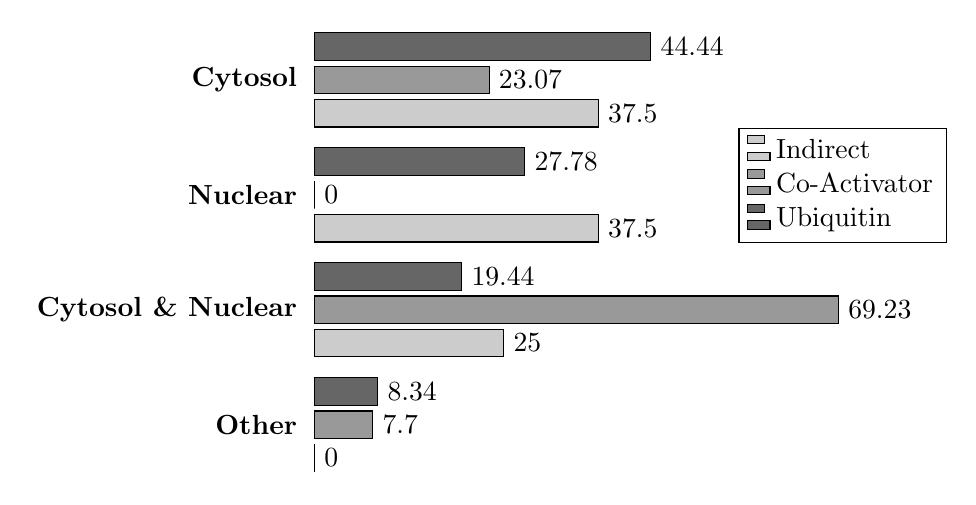
\begin{tikzpicture}
    \begin{axis}[
        xbar,
        y axis line style = {opacity=0},
        axis x line       = none,
        tickwidth         = 0pt,
        enlarge y limits  = 0.15,
        enlarge x limits  = 0.015,
        symbolic y coords = {Other, Cytosol \& Nuclear, Nuclear, Cytosol},
        nodes near coords,
        tick label style={font=\bfseries},
        legend style={
          area legend,
          at={(0.8,0.65)},
          anchor=west,
          legend cell align=left,
          legend columns=1},
      ]
          
      \addplot[black,fill=black!20,mark=none] coordinates {
        (0,Other)
        (25.00,Cytosol \& Nuclear)
        (37.50,Nuclear)
        (37.50,Cytosol)
      };
      \addplot[black,fill=black!40,mark=none] coordinates {
        (7.70,Other)
        (69.23,Cytosol \& Nuclear)
        (0,Nuclear)
        (23.07,Cytosol)
      };
      \addplot[black,fill=black!60,mark=none] coordinates {
        (8.34,Other)
        (19.44,Cytosol \& Nuclear)
        (27.78,Nuclear)
        (44.44,Cytosol)
      };
      
      \legend{Indirect, Co-Activator, Ubiquitin}
    \end{axis}
  \end{tikzpicture}
  \caption{Localization of UBE3A protein interactions (\%)}
\end{figure}
%%%%%%%%%%%%%%%%%%%%%%%%%%%%%%%%%%%%%%%%%%%%%%%%%%%%%%
